\documentclass[a4paper,10pt]{article}
\usepackage[utf8]{inputenc}

\usepackage{amsmath}
\usepackage{float}
\usepackage{graphicx}
\graphicspath{ {./images/} }

%opening
\title{Homework 1}
\author{Erivelton Gualter dos Santos}

\begin{document}

\date{}
\maketitle

%%%%%%%%%%%%%%%%%% Question 1 %%%%%%%%%%%%%%%%%%
\section{Question}

The circuit shown in the figure below contains a nonlinear inductor and is driven by a time-dependent current source. Suppose that the nonlinear inductor is described by $i_L =I_0\sin(k\phi_L)$, where $\phi_L$ is the magnet flux of the inductor and $I_0$ and $k$ are constants. Using $\phi_L$ and $v_C$ as state variables, find the state equations.

\hfill \break

Knowing the capacitor current is related to the capacitor voltage by 

\begin{equation}
 i_c(t) = C\frac{dv_c(t)}{dt} \label{eq:ic}
\end{equation}

and the inductor voltage is related to the inductor current by 

\begin{equation}
 v_l(t) = L\frac{di_l(t)}{dt} \label{eq:vl}
\end{equation}

and after choosing the state variables as $v_c$ and $\phi_l$, we can find the state space representation. 

Replacing the nonlinear inductor current in equation \ref{eq:vl}, we have:

\begin{eqnarray*}
 v_l(t) &= L\frac{d}{dt}(I_0\sin(k\phi_l))  \\
 &= LkI_0\cos(k\phi_l)\dot{\phi}_l
\end{eqnarray*}

as $v_l=v_c=v_R$, we can write the following equation in terms of state variables:

\begin{eqnarray}
 v_c(t) = LkI_0\cos(k\phi_l)\dot{\phi}_l \label{eq:dphi}
\end{eqnarray}

Applying Kirchhoff's current law (KCL) in the circuit, we hav e $i_c = i_s-i_l-i_R$. By replacing the respective quantities:

\begin{equation}
 i_c = i_s - I_0\sin(k\phi_l) - \frac{v_c}{R} \label{eq:ic2}
\end{equation}

Therefore, replacing equation \ref{eq:ic2} in equation \ref{eq:ic}: 

\begin{equation}
i_s - I_0\sin(k\phi_l) - \frac{v_c}{R} = C\frac{dv_c(t)}{dt} \label{eq:dvc}
\end{equation}

Finally, after reoordering the equations \ref{eq:dphi} and \ref{eq:dvc}:

\begin{equation}
  \begin{cases}
    \dot{v}_c = \frac{1}{C} \left(- \frac{v_c}{R} - I_0\sin(k\phi_l)+ i_s\right)\\
    \dot{\phi}_l = \frac{v_c}{LkI_0\cos(k\phi_l)}
  \end{cases}
\end{equation}
%%%%%%%%%%%%%%%%%% Question 2 %%%%%%%%%%%%%%%%%%
\section{Question}
Use Matlab/Simulink to simulate the stable electronic oscillator in Example 8 in Lecture 1. Choose two sets of initial conditions that are different from the ones on pages 28-30 in this lecture, and produce the phase plane (or XY plane) plots and
plot output responses with the various initial conditions. 
In your simulation, please choose $A=1.5$, $V_1 =V_2 =1$, $L=1$, $C=1F$, and $R=0.1\Omega$.

\begin{figure}[H]
 \begin{minipage}{.5\textwidth}
  \centering
  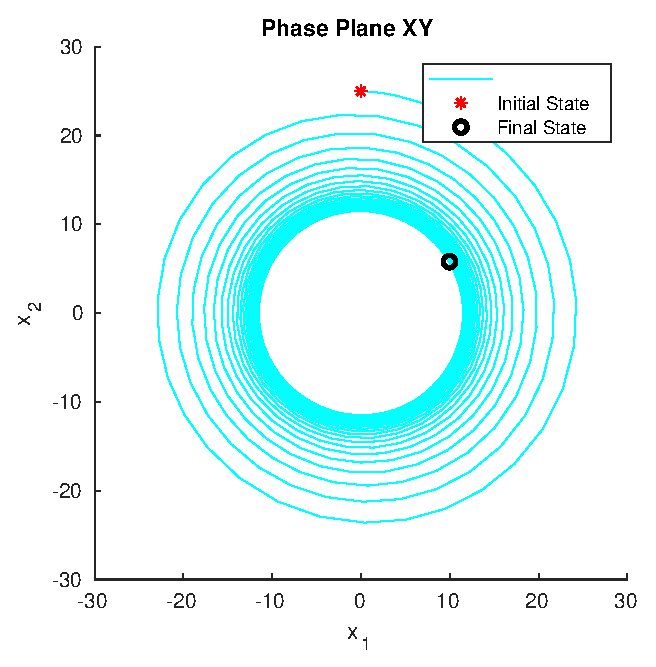
\includegraphics[width=.8\linewidth]{question2a.eps}
  \caption{Phase plane for $(0,30)$.} \label{fig:q2a}
 \end{minipage}
 \begin{minipage}{.5\textwidth}
  \centering
  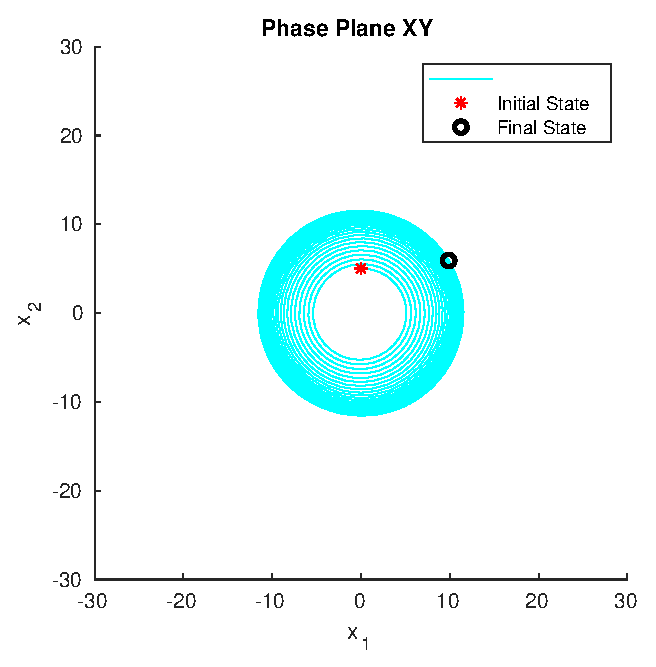
\includegraphics[width=.8\linewidth]{question2b.eps}
  \caption{Phase plane for $(0,5)$.} \label{fig:q2b}
 \end{minipage}
\end{figure}

%%%%%%%%%%%%%%%%%% Question 3 %%%%%%%%%%%%%%%%%%
\section{Question}
For the following system, find the equilibrium points and determine the type of each isolated equilibrium point:

\begin{eqnarray*}
\dot{x}_1 &= 2{x}_1 - {x}_1{x}_2 \\
\dot{x}_2 &= 2{x}^2_1 - {x}_2 
\end{eqnarray*}

By definition, the following equation must hold:

\begin{eqnarray}
0 &= 2{x}_1 - {x}_1{x}_2 \label{eq:3a} \\ 
0 &= 2{x}^2_1 - {x}_2   \label{eq:3b}
\end{eqnarray}

Replacing Equation \ref{eq:3b} in Equation \ref{eq:3a}, we have:

\begin{eqnarray*}
0 &= 2{x}_1 - 2{x}^3_1 \\
0 &= 2{x}_1(1 - {x}^2_1)
\end{eqnarray*}

Then, there are three solutions for $x_1$ and $x_2$

\begin{equation}
\begin{pmatrix}
x_{1e}\\x_{2e}
\end{pmatrix}=
\begin{bmatrix}
 0 & -1 & 1 \\
 0 & 2 & 2 
\end{bmatrix}
\end{equation}

\begin{figure}[H]
  \centering
  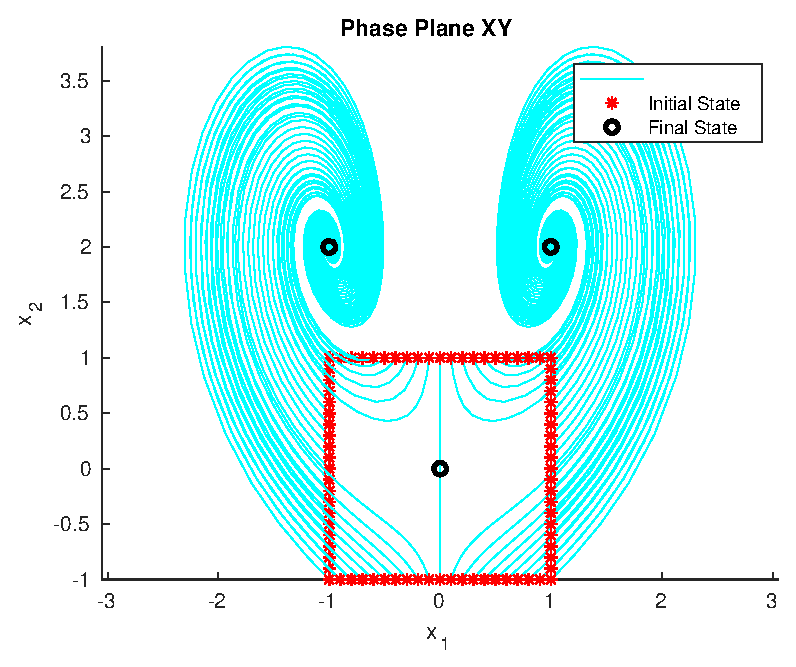
\includegraphics[width=.8\linewidth]{question3.eps}
  \caption{Phase plane for XY.} \label{fig:q3}
\end{figure}

%%%%%%%%%%%%%%%%%% Question 4 %%%%%%%%%%%%%%%%%%
\section{Question}
By plotting trajectories starting at different initial conditions, draw the phase portrait of the following LTI systems:

\begin{eqnarray}
\dot{x}_1 &= {x}_2 \\
\dot{x}_2 &= -10{x}_1-10{x}_2  
\end{eqnarray}

\begin{figure}[H]
  \centering
  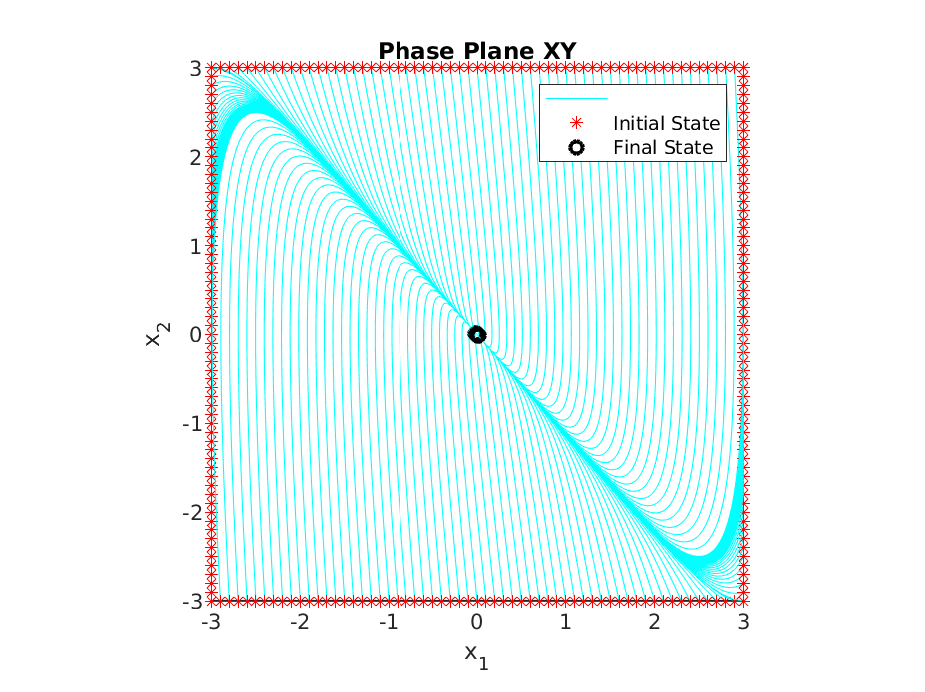
\includegraphics[width=.8\linewidth]{question4.eps}
  \caption{Phase plane for XY.} \label{fig:q4}
\end{figure}

%%%%%%%%%%%%%%%%%% Question 4 %%%%%%%%%%%%%%%%%%
\section{Question}
The phase portrait (or phase-plane plot) of the following system is shown below.
Mark the arrowheads and discuss the stability of each isolated equilibrium point


\begin{equation}
\dot{x}_1 = {x}_2 
\end{equation}

\begin{equation}
\dot{x}_2 = {x}_1-2\tan^{-1}({x}_1+{x}_2) 
\end{equation}

\end{document}
